% SPDX-FileCopyrightText: 2026 Cyprien PIERRE
% SPDX-License-Identifier: CC-BY-4.0
\documentclass[tikz,border=5pt]{standalone}
\usepackage[T1]{fontenc}
\usepackage{lmodern}
\usepackage{amsmath,amssymb}
\usetikzlibrary{arrows.meta}
\begin{document}
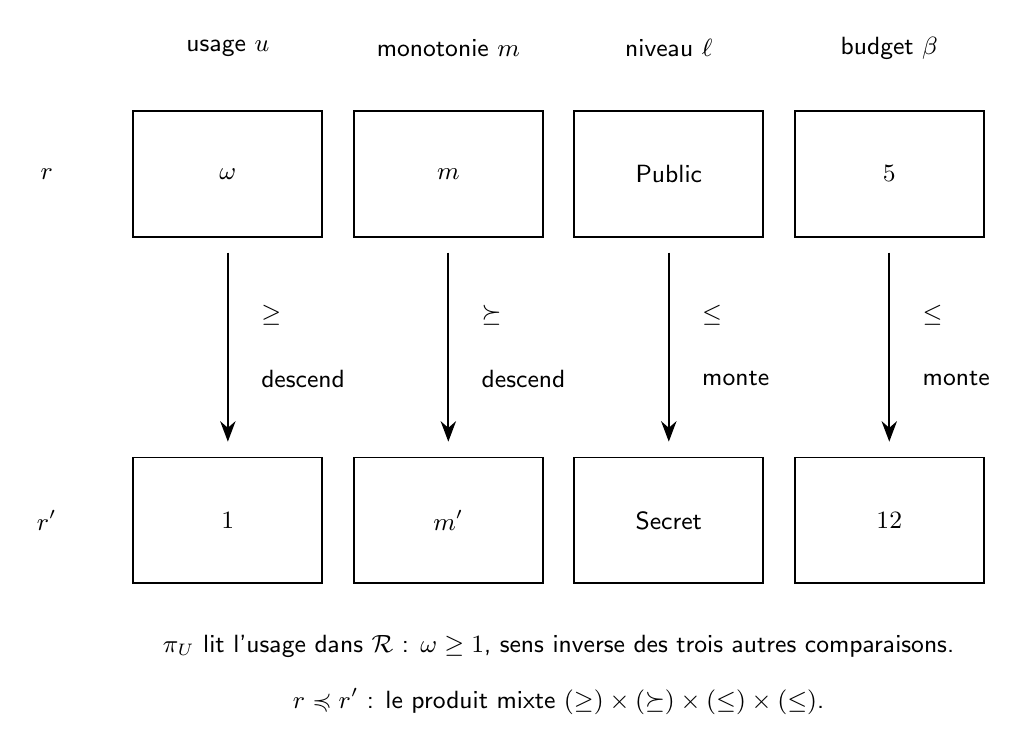
\begin{tikzpicture}[
  font=\sffamily\small,
  cell/.style={draw, line width=.65pt, minimum width=24mm, minimum height=16mm, align=center},
  arr/.style={-{Stealth[length=2.6mm]}, line width=.8pt}
]
% Component labels
\node at (33mm,86mm) {usage $u$};
\node at (61mm,86mm) {monotonie $m$};
\node at (89mm,86mm) {niveau $\ell$};
\node at (117mm,86mm) {budget $\beta$};

% Top quadruplet r
\node at (10mm,70mm) {$r$};
\node[cell] at (33mm,70mm) {$\omega$};
\node[cell] at (61mm,70mm) {$m$};
\node[cell] at (89mm,70mm) {Public};
\node[cell] at (117mm,70mm) {$5$};

% Bottom quadruplet r'
\node at (10mm,26mm) {$r'$};
\node[cell] at (33mm,26mm) {$1$};
\node[cell] at (61mm,26mm) {$m'$};
\node[cell] at (89mm,26mm) {Secret};
\node[cell] at (117mm,26mm) {$12$};

% Coercion arrows, one per component
\draw[arr] (33mm,60mm) -- (33mm,36mm);
\draw[arr] (61mm,60mm) -- (61mm,36mm);
\draw[arr] (89mm,60mm) -- (89mm,36mm);
\draw[arr] (117mm,60mm) -- (117mm,36mm);

% Relations and directions
\node[anchor=west] at (36mm,52mm) {$\geq$};
\node[anchor=west] at (36mm,44mm) {descend};
\node[anchor=west] at (64mm,52mm) {$\succeq$};
\node[anchor=west] at (64mm,44mm) {descend};
\node[anchor=west] at (92mm,52mm) {$\leq$};
\node[anchor=west] at (92mm,44mm) {monte};
\node[anchor=west] at (120mm,52mm) {$\leq$};
\node[anchor=west] at (120mm,44mm) {monte};

% The reversal read through pi_U
\node at (75mm,10mm) {$\pi_U$ lit l'usage dans $\mathcal{R}$ : $\omega \geq 1$, sens inverse des trois autres comparaisons.};
\node at (75mm,3mm) {$r \preccurlyeq r'$ : le produit mixte $({\geq}) \times ({\succeq}) \times ({\leq}) \times ({\leq})$.};
\end{tikzpicture}
\end{document}
